\chapter{Preliminaries}
\label{chap:prelim}

We begin with some basic definitions pertaining to reachability and parallelotopes. The definition of Bernstein polynomials and the reachable set computaion algorithm will be defined. Finally, an outline of the reachability algorithm given by \cite{dreossi2016parallelotope} for polynomial dynamical systems will be presented.

\section{Basic Definitions}
\label{sec:definitions}

As stated in the previous sections, this thesis pertains to the reachability analysis of dynamical systems. Roughly speaking, a dynamical system is governed by a set of differential equations such that the states of the system evolve according the solutions of the said differential equations.
%
The state of a system, denoted as $x$, lies in a domain $D \subseteq \reals^n$ where the solution to the differential equations is defined.
%
We restrict our attention to a specific definition of these dynamical systems:
%
\begin{definition}
A discrete-time nonlinear system is denoted as
\begin{equation}
  x^{+} = f(x)
\label{eq:sys}
\end{equation}
where $f: \reals^{n} \rightarrow \reals^{n}$ is a nonlinear function.
\end{definition}
%
 Intuitively, the function $f$ takes input a state of the system and outputs the next step of the system evolved according to the non-linear dynamics.
%
Here, the function $f$ generally represents some discretized version of some specified continuous non-linear dynamical systems. Recall that a dynamical system is considered \emph{linear} if its dynamics can be expressed as

$$
x' = Ax, \quad A \in \reals^{n \times n}
$$
%
Otherwise, we deem the system to be \emph{nonlinear}.
%
Hence, in particular, the function $f$ cannot be expressed as some matrix $A \in \reals^{n \times n}$.

Examples of prominent non-linear dynamical systems include the Lotka-Volterra predator-prey model \cite{wangersky1978lotka}, FitzHugh Neuron model \cite{fitzhugh1961impulses}, and recently introduced COVID19 disease model \cite{indiansuper2020supermodel}. Throughout this thesis, we discretize any continuous dynamics through the well-known Euler method. Thus, up to some error term of bounded degree, we can turn any non-linear system into the form given by Equation~\ref{eq:sys}.
%
\begin{example}
The SIR Epidemic model is a 3-dimensional dynamical system governed by the following continuous dynamics:
\begin{align} \label{eqn:sir}
    \begin{split}
        s' &= \beta \cdot s_k i_k \\
        i' &= \beta \cdot s_k i_k - \gamma \cdot i_k \\
        r' &= \gamma \cdot i_k
    \end{split}
\end{align}
where $s,i,r$ represent the fractions of a population of individuals designated as \textit{susceptible}, \textit{infected}, and \textit{recovered} respectively. There are two parameters, namely $\beta$ and $\gamma$, which influence the evolution of the system. $\beta$ is labeled as the contraction rate and $1/\gamma$ is the mean infective period.
%
Discretizing Equation~\ref{eqn:sir} according the Euler method yields the dynamics:
%
\begin{align} \label{eqn:discrete_sir}
    \begin{split}
        s_{k+1} &= s_k - (\beta \cdot s_k i_k)\cdot\Delta \\
        i_{k+1} &= i_k + (\beta \cdot s_k i_k - \gamma \cdot i_k)\cdot\Delta \\
        r_{k+1} &= r_k + (\gamma\cdot i_k)\cdot\Delta
    \end{split}
\end{align}
 Here, $\Delta$ is the discretization step and the index $k \in \mathbb{N}$ simply represents the current step.
%For the benchmarks, we set $\beta = 0.34$, $\gamma=0.05$, and $\Delta=0.5$.
%
Note the non-linear terms $s_ki_k$ which precludes the expression of the dynamics as a linear transformation.
\end{example}

The trajectory of a system that evolves according to Equation~\ref{eq:sys}, denoted as $\xi(x_0)$ is a sequence $x_0, x_1, \ldots $ where $x_{i+1} = f(x_i)$.
%
The $k^{th}$ element in this sequence $x_k$ is denoted as $\xi(x_0,k)$.

\begin{definition}
Given an initial set $\Theta \subseteq \reals^n$, the \emph{reachable set at step $k$}, denoted as $\Theta_k$ is defined as
\begin{equation}
  \Theta_k = \{ \xi(x,k)\: | \: x \in \Theta\}
\label{eq:reachset}
\end{equation}
If we set the number of steps to be some $n \in \mathbb{N}$, we say the \emph{reachable set} is
\begin{equation}
  \Theta = \bigcup_{i=1}^n \Theta_i
\end{equation}
\end{definition}

%
We will see in a future section an example of the reachable set of the discretized SIR model presented in Equation~\ref{eqn:discrete_sir}.


\section{Parallelotope-based Reachability}

\subsection{Parallelotopes}
\label{sec:parallelotope}
A parallelotope $P$ is a set of states in $\mathbb{R}^{n}$ captured by the tuple $\langle \Lambda, c\rangle$ where $\Lambda \in \mathbb{R}^{2n \times n}$ is a matrix and $ç$ is a column vector. We impose the condition that $\Lambda_{i+n} = -\Lambda_{i}$ for all $i \in \{1, \ldots, n\}$ such that
%
\begin{equation}
\label{eq:halfspace}
x \in P \mbox{ if and only if } \Lambda x \leq c.
\end{equation}
We deem $\Lambda$ as the \emph{template direction matrix} where $\Lambda_i$ denotes the $i^{th}$ row of $\Lambda$ called the \emph{$i^{th}$ template direction}. The column vector $c$ is called the \emph{offset vector} with $c_i$ denoting the $i^{th}$ element of $c$.
%
If we unpack Equation~\ref{eq:halfspace}, we can re-express the inequalities as a conjection of half-space constraints. If we define $c_{u} = [c_1, c_2, \cdots, c_n]^T$ and $c_{l} = [c_{n+1}, c_{n+2}, \cdots, c_{2n}]^T$, then Equation~\ref{eq:halfspace} tells us that:
%
\begin{align*}
  & \Lambda_i x \leq (c_u)_i \\
  -& \Lambda_i x \leq (c_l)_i
\end{align*}
%
Additionally, the definition of the paralleotope above requires that for each of $n$ ``postive" directions, there must exist a corresponding ``negative" direction. This is encoded into the template matrix $\Lambda$ by the condition $\Lambda_{i+n} = -\Lambda_{i}$. However, by the observation made above, we only need to keep the positive directions and divide our offset vector into equal components with the top half encoding the offsets for the positive directions and the bottom half encoding the offsets for the negative directions.
%
Combining these remarks yields the \emph{half-space representation} of parallelotope $P$.
%
\begin{definition}
\label{def:halfspace_def}
The half-space representation of parallelotope $P$ is tuple  $\langle \Lambda, c_l, c_u \rangle$ where $\Lambda \in \mathbb{R}^{n \times n}$ and $c_l, c_u \in \reals^n$
such that
\begin{equation}
\label{eq:halfspaceconst}
P =\{x ~|~ c_l \leq \Lambda x \leq c_u\}
\end{equation}
\end{definition}


\begin{example}
\label{ex:simple_ptope}
Consider the 2D plane, namely $\reals^2$. We can construct a couple of simple examples of parallelotopes. First, if we define our parallelotope's template direction matrix to be
%come back to this
\end{example}


\noindent Alternatively, a parallelotope can also be represented in a \emph{generator representation}
%
\begin{definition}
The generator representation of a parallelotope $P$ is a tuple of vectors $\langle v, g_1, \ldots, g_n\rangle$ such that $v,g_1, \cdots g_n \in \reals^n$. The vector  $v \in \mathbb{R}^n$ is called the \emph{anchor} and the $g_i \in \mathbb{R}^n$, are called the \emph{generators}. The parallelotope is defined as the set:
$$
P := \{ x ~|~ \exists \alpha_1, \ldots, \alpha_n \in [0,1], \; x = v + \sum_{i=1}^n \alpha_i g_i \}
$$
\end{definition}
%
\noindent This representation is very similar to Zonotopes~\cite{girard2005reachability,althoff2010computing} and Star sets~\cite{duggirala2016parsimonious}.
%
In particular, a parallelotope is a special case of a zonotope where the number of generators is exactly the dimension of the system $n$.

There is a simple method to convert from the half-space representation of $P$ to its generator representation.
%
Obtain vertex $v_1$ by solving the linear equation $\Lambda x = c_{l}$.
%
The $j+1$ vertex is obtained by solving the linear equation $\Lambda x = \mu_{j}$ where $\mu_{j}[i] = c_{l}[i]$ when $i \neq j$ and $\mu_{j}[j] = c_{u}[j]$.
%
The anchor $v$ of the parallelotope is the vertex $v_1$ and the generators will be $g_{i} = v_{i+1} - v_{1}$. Refer to \cite{dang2014parameter} for a more detailed exposition of this procedure.

%
As a final remark, notice that for a parallelotope $P$, the generator representation also defines an affine transformation that maps $[0,1]^{n}$ to $P$.
%
Let us denote this affine transformation associated to $P$ as $T_P$.

\begin{example}
\label{ex:ptope}
Once again, consider the space $\reals^2$ and the parallelotope $P$ given in half-plane representation as $0 \leq x-y \leq 1$, $0 \leq y \leq 1$.
%
This is a parallelotope with vertices at $(0,0)$, $(1,0)$, $(2,1)$, and $(1,1)$.
%
In the half-space representation, the template directions of the parallelotope $P$ are given by the directions $[1, -1]$ and $[0, 1]$.
%
The half-space representation in matrix form is given as follows:

\begin{equation}
  \begin{bmatrix} 0 \\ 0 \end{bmatrix} \leq \begin{bmatrix}  1 & -1 \\ 0 &  1 \end{bmatrix}  \begin{bmatrix} x \\ y \end{bmatrix} \leq \begin{bmatrix} 1 \\ 1 \end{bmatrix}. \label{eq:ptopeexample}
\end{equation}

To compute the generator representation of $P$, we need to compute the \emph{anchor} and the \emph{generators}.
%
The anchor is obtained by solving the linear equations $x-y = 0, y = 0$.
%
Therefore, the anchor $a$ is the vertex at origin $(0,0)$
%
To compute the two generators of the parallelotope, we compute two vertices of the parallelotope.
%
Vertex $v_1$ is obtained by solving the linear equations $x - y = 1, y = 0$.
%
Therefore, vertex $v_1$ is the vertex $(1,0)$.
%
Similarly, vertex $v_2$ is obtained by solving the linear equations $x-y = 0, y = 1$.
%
Therefore, $v_2$ is the vertex $(1,1)$.
%
The generator $g_1$ is the vector $v_1 - a$, that is $(1,0)- (0,0) = (1,0)$
%
The generator $g_2$ is the vector $v_2 - a$, that is $(1,1) - (0,0) = (1,1)$.
%
Therefore, all the points in the paralellotope can be written as $(x,y) = (0,0) + \alpha_1 (1,0) + \alpha_2(1,1)$, $\alpha_1, \alpha_2 \in [0,1]$.
\end{example}
%
%We denote this affine transformation as $T_{p}$.
%
\begin{definition}
A parallelotope bundle $Q$ is a set of parallelotopes $\{P_0, \ldots, P_m\}$ such that
  $$ Q = \bigcap_{i=1}^{m}P_i $$.
\end{definition}

\begin{remark}
There is a slight abuse of notation above where we refer to the parallelotope bundle $Q$ as both the set of parallelotopes and the region in $\reals^n$ of the intersection of all the parallelotopes $P_i$. To specify the \emph{set of parallelotopes} which consists the bundle, we will write
$$
\mathcal{P}(Q) = \{P_0, \ldots, P_m\}
$$
\end{remark}

%
\noindent This parallelotope bundle will be the geometric data structure which will enclose the region we compute to be the approximation of the exact reachable set.

\subsection{Bernstein Polynomials}
\label{sec:bernstein}
In this section, we define Bernstein polynomials and state some of their enclosure properties. A \emph{multi-index} ${\bf i}$ of length $n$ is defined as tuple of $n$ elements ${\bf i} = (i_1,\cdots, i_n)$ such that each $i_k \in \mathbb{N}$. Furthermore, we order the multi-indices as follows: if ${\bf i}$ and ${\bf j}$ are two multi-indices of length $n$, then
\[
  {\bf i} \leq {\bf j} \iff i_k \leq j_k, \quad 1 \leq  k \leq n
\]
Finally, we generalize the product of binomial coefficients as:
\[
  \binom{\boldi}{\boldj} := \prod_{k=1}^n \binom{i_k}{j_k}
\]
%
Given two multi-indices $\boldi$ and $\boldd$ of size $n$, where $\boldi \leq \boldd$, the Bernstein basis polynomial of degree $\boldd$ and index $\boldi$ is defined as:
\begin{equation}
\label{eq:bernstein_basis_poly}
\mathcal{B}_{(\boldi,\boldd)}(\boldx) = \beta_{i_1,d_1}(x_1) \beta_{i_2,d_2}(x_2)\ldots \beta_{i_n,d_n}(x_n).
\end{equation}
%
where for $i,d,x \in \reals$:
%
\begin{equation}
\beta_{i,d}(x) = \binom{d}{i}x^{i}(1-x)^{d - i}
\end{equation}
%
Let $p: \reals^n \rightarrow \reals$ of be a real polynomial of degree at most $\boldd$. We can express $p$ as a linear combination of monomials of degree at most $\boldd$:
\[
p(\boldx) = \sum_{\boldi \leq \boldd} a_\boldi \cdot \boldx^\boldi
\]
where $\boldx^\boldi$ represents the monomial $x_1^{i_1}x_2^{i_2}\cdots x_n^{i_n}$. Every such real polynomial $p$ can be represented as linear combination of Bernstein basis polynomials of of degree $\boldd$:
%
\begin{equation}
  p(\boldx) = \sum_{\boldi \leq \boldd} b_{\boldi} \cdot \mathcal{B}_{(\boldi,\boldd)}(\boldx)
\end{equation}
where $b_\boldi$ denotes the \emph{$\boldi^{th}$ Bernstein Coefficient}:

\begin{equation}
b_{\boldi} = \sum_{\boldj \leq \boldi} \frac{\binom{\boldi}{\boldj}}{\binom{\boldd}{\boldj}}\cdot a_{\boldj}
\end{equation}
%
\noindent In other words, given a polynomial $p(x_1,\ldots,x_n) = \sum_{j \in J} a_j {\bf x}_{j}$ where $J$ is a set of multi-indices iterating through the degrees found in $p$ with $a_j \in \mathbb{R}$, then $p(x_1,\ldots,x_n)$ can be converted into its counterpart under the Bernstein basis, $p(x_1,\ldots,x_n) = \sum_{j \in J} b_j \mathcal{B}_j $ where $b_j$ are the corresponding Bernstein coefficients.

The primary advantage of the Bernstein representation of a polynomial $p(x_1,...,x_n)$ is that an upper bound on the supremum and lower bound on the infimum of $p(x_1,...,x_n)$ in $[0,1]^{n}$ can be computed purely by observing the coefficients of the polynomial in the Bernstein basis. Specifically, the upper and lower bounds of $p(x_1,\ldots,x_n)$ over $[0,1]^n$ are bounded by the Bernstein coefficients. We state this as a property without proof.
%
\begin{property} (Enclosure Property)
  \label{prop:bern_enclosure}
  Let $p: \reals^n \rightarrow \reals$ be a real mutlivarite polynomial of degree $\boldd$, and let $p(\boldx) = \sum_{\boldi \leq \boldd} b_\boldi \cdot \mathcal{B}_{(\boldi,\boldd)}(\boldx)$ be the Bernstein expansion of $p$, then
  $$
  \min_{\boldi \leq \boldd} \{b_\boldi\} ~~\leq~~ \inf_{x \in [0,1]^n} p(x) ~~~~~\leq~~~~ \sup_{x \in [0,1]^{n}} p(x) ~~\leq~~ \max_{\boldi \leq \boldd} \{b_\boldi\}
  $$
\end{property}


As mentioned earlier, a parallelotope $P$ can also be represented as an affine transformation $T_{p}$ from $[0,1]^{n}$ to $P$.
%
Therefore, upper bounds on the suprenum of a polynomial function $p$ over $P$ is equivalent to upper bound of $p \circ T_{p}$ over $[0,1]^{n}$.
%
A similar argument follows for the lower bound on the infimum.
%
The crux of the reachability algorithm involves exploiting this property of Bernstein polynomials to approximate the solution of certain non-linear optimization problem invovilng polynomial predicates over the unitbox, $[0,1]^n$.
%
We will cover this algorithm in the upcoming section.
%
For a more rigorous exposition on Bernstein polynomials and Property~\ref{prop:bern_enclosure}, refer to \cite{garloff2003bernstein}.

\subsection{The Static Algorithm}
\label{sec:static}

We will end with an outline of the static algorithm first investigated in works \cite{dang2012reachability, dreossi2016parallelotope}. As mentioned in the previous section, the building block of the reachability algorithm relies on approximate solutions to a non-linear optimization problem over the unit-box domain. Consider a non-linear function $h : \reals^n \rightarrow \reals$. The most general form of this optimization problem can be expressed as:
%
\begin{eqnarray}
  \max ~ h(x) \label{eq:maxsup}\\
  s.t. ~~ x \in [0,1]^{n}.\nonumber
\end{eqnarray}

In the static algorithm, the user manually specifies the number of parallelotopes and a set of static directions for each parallelotope. In other words, the user must specify the template matrix $\Lambda$ and its corresponding offset vector $c$ for each parallelotope $P = \langle \Lambda, c\rangle$ contained in the bundle \emph{before} the computation begins.

We now proceed to formally describe the static algorithm.
%
First, a small remark on the template matrix of the parallelotopes $P_i$ contained in some bundle $Q$. It is possible that some of the parallelotopes share the same template matrix directions.
%
 In other words, for $P_i = \langle \Lambda^{P_i}, c^{P_i} \rangle, P_j = \langle \Lambda^{P_j}, c^{P_j} \rangle$ such that $P_i, P_j \in \ptopeset{Q}$, there could exist some $k$ such that $\Lambda^{P_i}_k = \Lambda^{P_j}_k$ as row vectors.
%
Thus, a more compact method of encoding the bundle is by taking the \emph{distinct} template directions as rows of a new template matrix $\Lambda^Q$ along with its corresponding offset vector $c^Q$.
%
To distinguish between the distinct parallelotopes contained in the bundle, we add a new matrix called the \emph{bundle index matrix}, $\T^Q \in \mathbb{N}^{p \times n}$, such that $\T^Q_i$ is a vector of row indices of $\Lambda^Q$ which specify the template directions defining parallelotope $P_i \in \ptopeset{Q}$.
%
The number of rows will thus be the number of distinct parallelotopes contained in the bundle $p = |\ptopeset{Q}|$.
%
\begin{remark}
If none of the paralleotopes $P_i \in \ptopeset{Q}$ share common template directions, then $\Lambda^Q$ will simply be the template direction matrices $\{\Lambda^P\}_{P \in \ptopeset{Q}}$ concatenated along their rows. This will generally be the matrix generated by the dynamic algorithm we will outline in a future section.
\end{remark}
%
\begin{example}
Set our space to be $\reals^2$. Consider the parallelotope bundle $Q$ containing three individual parallelotopes $P_0, P_1, P_2$ with the following template direction matrices:
  \begin{equation*}
    \Lambda^{P_0}  = \begin{bmatrix}
                  1 & 0 \\
                  0 & 1
                  \end{bmatrix}, \quad
    \Lambda^{P_1}  = \begin{bmatrix}
                    1 & 0 \\
                    1 & 1
                    \end{bmatrix}, \quad
    \Lambda^{P_2} = \begin{bmatrix*}[r]
                    0 & 1 \\
                   -1 & 1
                    \end{bmatrix*}
  \end{equation*}
  The associated template direction matrix and bundle index matrix for $Q$ will then be defined as follows:
  \begin{equation*}
    \Lambda^{Q} = \begin{bmatrix*}[r]
                  1 & 0 \\
                  0 & 1 \\
                  1 & 1 \\
                  -1 & 1
                  \end{bmatrix*}, \quad
                  \T^Q = \begin{bmatrix}
                          0 & 1 \\
                          0 & 2 \\
                          1 & 3
                         \end{bmatrix}
  \end{equation*}
\end{example}

\noindent Another input to the algorithm is the initial parallelotope bundle, given as $Q$. When the initial set is a box, $P_0$ will be defined by the axis-aligned template directions.

The output of the algorithm is, for each step $k$, the set $\overline\Theta_k$, which is an over-approximation of the reachable set at step $k$, $\Theta_k \subseteq \overline\Theta_k$. The total over-approximation of the reachable set for a finite number of steps $n$ will be $\overline\Theta = \cup_{k=1}^n \overline\Theta_k$.
%
The high-level pseudo-code is written in Algorithm~\ref{alg:old}.


%-----------------------------------------------------------------------------------------------------------------------------------------------------------------

\begin{figure}[t!]

\begin{algorithm}[H]
  \SetKwInput{KwInput}{Input}
  \SetKwInput{KwOutput}{Output}
  \SetKwFunction{AppendPCA}{AppendNewPCATemplates}
  \SetKwFunction{AppendLin}{AppendNewLinAppTemplates}
  \SetKwFunction{TransformBund}{TransformBundle}
  \SetKwFunction{UpdateTemp}{UpdateTemplates}
  \SetKwFunction{GetSupp}{GetSupportPoints}
  \SetKwFunction{PropPoints}{PropagatePointsOneStep}
  \SetKwFunction{PCA}{PCA}
  \SetKwFunction{ApproxLinearTrans}{ApproxLinearTrans}
  \SetKwFunction{SetLifeSpan}{SetLifeSpan}
  \SetKwFunction{AddTemptoBund}{AddTemplateToBundle}
  \SetKwFunction{RemoveTemp}{RemoveTempFromBund}
  \SetKwProg{Fun}{Proc}{:}{}

\SetAlgoLined
\DontPrintSemicolon

\KwInput{Dynamics $f$, Initial Parallelotope $P_0$, Step Bound $S$, Template Dirs $\Lambda$, indexes for parallelotopes $I$}
\KwOutput{Reachable Set Overapproximation $\overline\Theta_k$ for each step $k$}
$Q_0 = \{ P_0 \}$ \;
 \For{$k \in [1, 2, \ldots, S]$}{
    $Q_k$ = \TransformBund($f$, $Q_{k-1}$, $\Lambda$) \;
   $\overline\Theta_k = Q_k$ \;
 }
 \Return{$\overline\Theta_1 \ldots \overline\Theta_S$} \;
 \;
 %
 \Fun{\TransformBund{$f$, $Q$, $\Lambda$}}{
   $Q' \gets \{\}$; $c_{u} \gets +\infty$; $c_{l} \gets -\infty$\;
   \For{each parallelotope $P$ in $Q$}{
     % $\tup{\T, c_{l}, c_{u}} \gets \mathsf{half-spaceRepresentation}(P)$\;
     $\langle v, G \rangle \gets \mathsf{generatorRepresentation}(P)$\;
     \For{each template direction $\Lambda_i$ in the template directions $\Lambda$ }{
       $c_{u}'[i] \gets \mathsf{min}\{ \mathsf{optBox(\Lambda_{i} \cdot f)}, c_{u}'[i] \}$ (Equation~\ref{eq:maxalpha})\;
       $c_{l}'[i] \gets \mathsf{max}\{ -1 \times \mathsf{optBox(-1\times \Lambda_{i} \cdot f)}, c_{l}'[i] \}$\;
     }
   }
   Construct parallelotopes $P_{1}', \ldots, P_{k}'$ from $\Lambda, c_{l}', c_{u}'$ and indexes from $I$ \;

   $Q' \gets \{P_{1}', \ldots, P_{k}'\}$ \;
   \Return{$Q'$}
 }
\end{algorithm}
\caption{Reachable set computation using manual and static templates.}
\label{alg:old}
\end{figure}



%-----------------------------------------------------------------------------------------------------------------------------------------------------------------


The algorithm simply calls $\tbundle$ for each step, producing a new parallelotope bundle computed from the previous step's bundle.
%
To compute the image of $Q$, the algorithm computes the upper and lower bounds of $f(x)$ with respect to each template direction $\Lambda_i^Q$.
%
Since computing the maximum value of $f(x)$ along each template direction over the intersection of the entire bundle $Q$ in one shot is computationally difficult, the algorithm instead computes the maximum value over each of the constituent parallelotopes and uses the minimum of all these maximum values.

The $\tbundle$  operation works as follows.
%
Consider a parallelotope $P$ in the bundle $Q$.
%
% and half-space representation as $\tup{\T, c_{l}, c_{u}$.
Given a template direction $\Lambda_i^Q$, the maximum value of $\Lambda_{i}^Q \cdot f(x)$ for all $x \in Q$ is less than or equal to the maximum value of $\Lambda_{i}^P \cdot f(x)$ for all $x \in P$ if $\Lambda_i^Q$ is a row in $\Lambda^P$.
%
Similar argument holds for the minimum value of $\Lambda_{i}^Q \cdot f(x)$ for all $x \in Q$.
%
Observe that these inequalities hold by virtue of the fact that $Q \subseteq P$ by definition.
%
To describe this more formally: if $\lambda^Q_i = \{ P \in \ptopeset{Q} ~|~ \Lambda_i^Q = \Lambda_k^P \text{ for some } k \}$, then
%
\begin{align}
    & \max_{x \in Q}{\Lambda_{i}^Q \cdot f(x)} \leq \min_{P \in \lambda^Q_i} {\max_{x \in P}{\Lambda_{i}^P \cdot f(x)}}  \label{eq:max_over_ptopes}
 \\
    & \max_{P \in \lambda^Q_i} {\min_{x \in P}{\Lambda_{i}^P \cdot f(x)}} \leq \min_{x \in Q}{\Lambda_{i}^Q \cdot f(x)} \label{eq:min_over_ptopes}
\end{align}

%
% We would like to compute the image of the parallelotope $P$ with respect to the non-linear transformation $f(x)$.
%
% That is, we would like to compute $P'$ such that $\forall x \in P, f(x) \in P'$.
%
% Given that current techniques use static template directions, the parallelotope $P'$ also uses the template directions $\T^{P}$.
%
\noindent Hence, to compute the upper and lower bounds of each template direction $\Lambda_{i} f(x)$ for all $x \in P$, we must find a solution to the following optimization problem:
%
\begin{eqnarray}
  \max ~ \Lambda_i^{P} \cdot f(x) \label{eq:maxf}\\
  s.t. ~~ x \in P.\nonumber
\end{eqnarray}
%
\noindent Note that $\Lambda_i^{P} \cdot f(x)$ is a dot product between the row vector $\Lambda_i^{P}$ and the component-wise dynamics of $f(x)$. This is similar to the method of computing support functions over convex sets \cite{boyd2004convex}.


By Definition \ref{def:generator_def}, all the states in $P$ can be expressed as a vector summation of an anchor and a convex combination of generators.
%
Let  $\langle v, g_1, \cdots, g_n \rangle$ be the generator representation of $P$.
%
The optimization problem given in Equation~\ref{eq:maxf} would then transform as follows.

\begin{eqnarray}
  \max ~ \Lambda_i^P \cdot f(a + \Sigma_{i=1}^{n} \alpha_i g_i) \label{eq:maxalpha}\\
  s.t. ~~ \overline\alpha \in [0,1]^{n}.\nonumber
\end{eqnarray}

Equation~\ref{eq:maxalpha} is a form of $\mathsf{optBox(\Lambda_{i} \cdot f)}$ over $[0,1]^n$.
%
One can compute an upper-bound to this non-linear optimization by computing the Bernstein coefficients of $\Lambda_i \cdot f(a + \Sigma_{i=1}^{n} \alpha_i g_i)$ and taking the maximum and minimum coefficients as shown in Property~\ref{prop:bern_enclosure}.
%
Similarly, we compute the lower-bound of $\Lambda_{i}\cdot f(x)$ for all $x \in P$ by computing the upper-bound of $-1 \times \Lambda_{i}\cdot f(x)$.
%
\begin{remark}
The original algorithm using Bernstein expansion proposed by \cite{dreossi2016parallelotope} assumed polynomial dynamics i.e $f$ is polynomial in the system variables.
%
This is to ensure that a $\Lambda_{i}\cdot f(x)$ is a polynomial after the composition shown in Equation \ref{eq:maxalpha}. Proper Bernstein expansion of this polynomial allows us to exploit the enclosure property of Bernstein coefficients. However, the use of other non-linear optimization solvers, such as Kodiak \cite{kodiak}, allows us to use more general dynamics involving trigonometric and root functions. A Taylor expansion of any analytic function can also be truncated to some suffciently large degree to admit a power series expansion.
\end{remark}

We iterate this process (i.e., computing the upper and lower bound of $\Lambda^Q_{i}\cdot f(x)$) for each parallelotope in the bundle $Q$ according to Equation \ref{eq:max_over_ptopes} and Equation \ref{eq:min_over_ptopes}).
%
% Observe that the role of the parallelotopes in the bundle is to compute an upper bound on the maximum value of $T_{i}f(x)$ by expanding the domain from $Q$ to the corresponding parallelotope $P$.
%
Therefore, the tightest upper bound on $\Lambda^Q_{i}\cdot f(x)$ over $Q$ is the least of the upper-bounds computed from each of the parallelotopes.
%
A similar argument holds for lower bounds of $\Lambda^Q_{i}\cdot f(x)$ over $Q$.
%
%\begin{figure}
%\subfloat[A single ptope]{
%  \begin{tikzpicture}
%    \draw (0,0) -- (-1,2) -- (3,2) -- (4,0) -- cycle;
%    \node at (1.5,1) {$P$};
%    \draw[->, very thick] (5,1) -- (7,1) node[above, midway] {$f$};
%    \draw (10,0) .. controls (7,1) ..(9,2) .. controls (10, 1).. (11,2) .. controls (14,1) .. (14,0) .. controls (11,-1) .. cycle;
%    \node at (11,0.75) {$f(P)$};
%  \end{tikzpicture}
%}
%\caption{Diagrams for the effect of the non-linear optimization procedure.}
%\end{figure}
%
Therefore, the image of the bundle $Q$ will be the bundle $Q'$ where the upper and lower-bounds for templates directions are obtained by solving a series of non-linear optimization problems of the form presented in Equation~\ref{eq:maxf}.

% TODO: Expound more on the menaings of constructing ptopes from the bundle index matrix.

Finally, once the loop on step two of Algorithm~\ref{alg:old} halts at step $S$, the outputted reachable set will be the computed over-approximations $\overline\Theta_1, \cdots, \overline\Theta_S$. As step four within the loop implies, this is simply the image bundles $Q'$ returned by our $\tbundle$ procedure.

\def \reachplotwidth {1.3}

\begin{example}
\label{ex:sir_kaa}
  We return to the SIR model briefly treated in Section \ref{sec:definitions}. Figure~\ref{fig:kaa_sir} shows the reachable set computed with the static algorithm and plotted using the following parameters:
  \begin{itemize}
    \item The parameters of the model are set to $\beta = 0.34$ and $\gamma = 0.05$. The discretization step is set to $\Delta = 0.1$.
    \item The parallelotope only has one static parallelotope, namely the initial box. This shows that our template matrix for $P$ is
        \begin{equation*}
          \Lambda^Q = \begin{bmatrix}
                      1 & 0 & 0 \\
                      0 & 1 & 0 \\
                      0 & 0 & 1
                      \end{bmatrix}
                      \quad
          \T^Q = \begin{bmatrix}
                      0 & 1 & 2 \\
                      \end{bmatrix}
        \end{equation*}
        %
        \begin{equation*}
            c_l^P = \begin{bmatrix} -0.79 & -0.19 & 0 \end{bmatrix}^T \quad c_u^P = \begin{bmatrix} 0.8 & 0.2 & 0 \end{bmatrix}^T
        \end{equation*}
    \item We set the number of time steps $S = 300$.
  \end{itemize}

  \begin{figure}[h!]
    \hspace*{-2.4cm}
    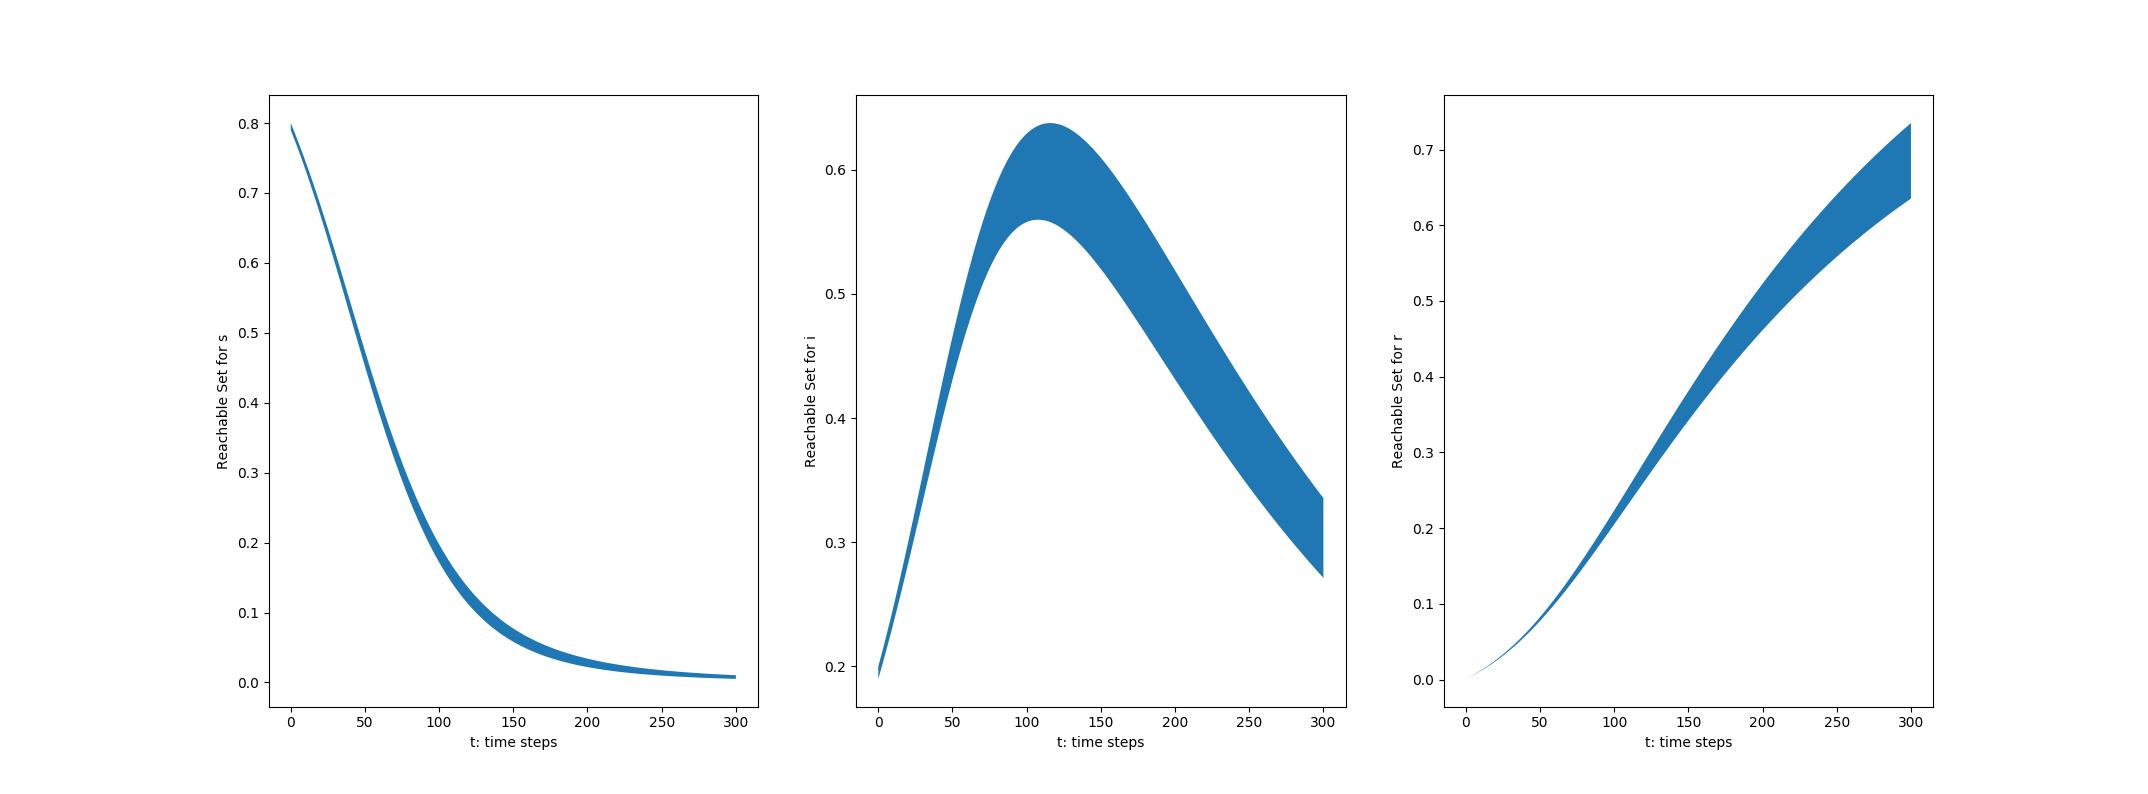
\includegraphics[width=\reachplotwidth\textwidth]{figures/SIRProj.png}
    \caption{Projection of Reachable Set of SIR propagated 300 steps in time.}
    \label{fig:kaa_sir}
  \end{figure}

  There a few points worth noting here. First, by the discussion leading to Definition~\ref{def:halfspace_def}, the initial set would be the box $[0.79,0.8] \times [0.19, 0.2] \times 0$. This can be interpreted as initializing the model such that $79-80\%$ of the population is susceptible (not yet infected) with $19-20\%$ of the population is infected. As the simulation is beginning, no percentage of the population has recovered from the disease. Hence, the third parameter $r$ is set to zero.
  %
  Second, since we only have the axis-aligned parallelotope in our initial bundle, the matrix $\T^Q$ will consist of only one row indicing the axis-aligned directions expressed as distinct rows in $\Lambda^Q$.
\end{example}

\begin{example}
\label{ex:phos}
To include an example of a higher-dimensional non-linear system, we introduce the Phosporaley model. The Phosphoraley model describes a certain cellular regulatory system. It is captured by seven variables governed by the discretized dynamics stated in Figure \ref{fig:phos_dynamics}.

\begin{center}
  \begin{equation*}
    \begin{cases}
        x^1_{k+1} &= x^1_k + ( -\alpha \cdot x^1_k + \beta \cdot x^3_k x^4_k)\cdot \Delta \\
        x^2_{k+1} &= x^2_k + (  \alpha\cdot  x^1_k - x^2_k)\cdot \Delta \\
        x^3_{k+1} &= x^3_k + ( x^2_k - \beta \cdot x^3_k x^4_k)\cdot \Delta \\
        x^4_{k+1} &= x^4_k + ( \beta \cdot x^5_k x^6_k - \beta \cdot x^3_k x^4_k)\cdot \Delta \\
        x^5_{k+1} &= x^5_k + ( -\beta \cdot x^5_k x^6_k + \beta \cdot x^3_k x^4_k)\cdot \Delta \\
        x^6_{k+1} &= x^6_k + ( \alpha\cdot  x^7_k - \beta \cdot x^5_k x^6_k)\cdot \Delta \\
        x^7_{k+1} &= x^7_k + ( -\alpha\cdot  x^7_k + \beta \cdot  x^5_k x^6_k)\cdot \Delta
    \end{cases}
  \end{equation*}
  \label{fig:phos_dynamics}
  \captionof{figure}{Discretized Dynamics of Phosphorlay Model.}
\end{center}
%
Here, we set the two parameters $\alpha,\beta$ as $\alpha=0.5$ and $\beta=5$. The discretization step is set to $\Delta =0.01$ and we propagate the reachble set for $S=300$ time steps. Additionally, the initial box is set to be $[1.00,1.01]^7 \times [-100, 100]$. Under these parameters, Figure \ref{fig:kaa_phos} depicts the projection of the reachable set on the first three variables $x_1, x_2, x_3$. The relevant matrices are defined as:

\begin{figure}[t!]
  \hspace*{-2.4cm}
  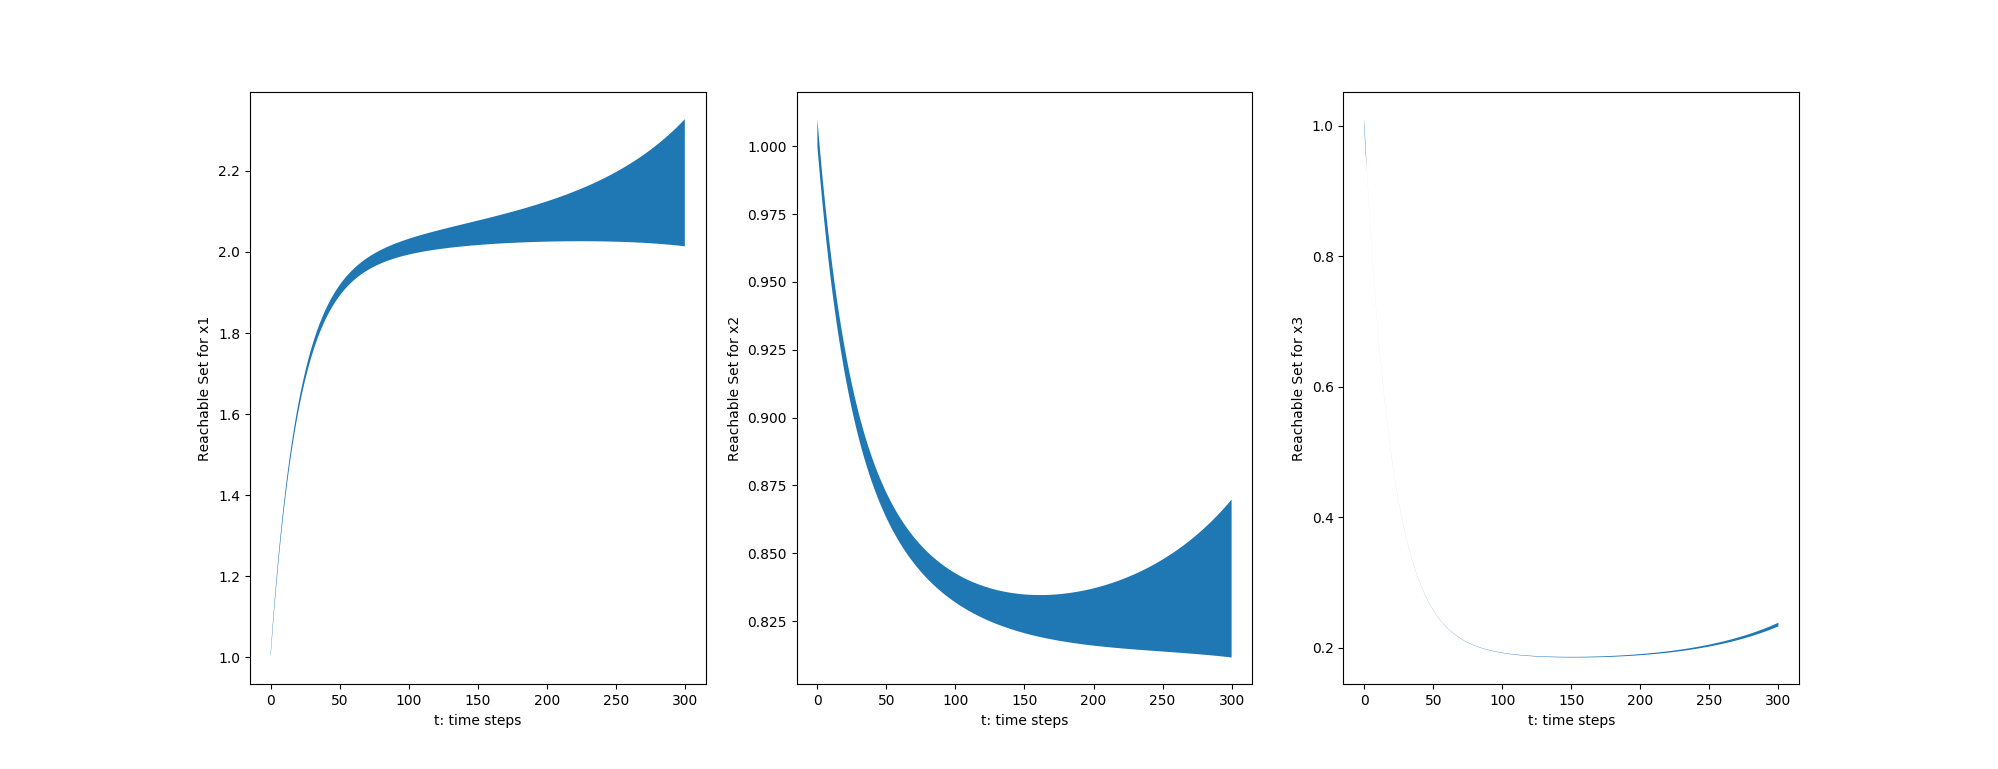
\includegraphics[width=\reachplotwidth\textwidth]{figures/PhosporlayProjOn X_1, X_2, X_3.png}
  \caption{Projection of Reachable Set of the Phosporaley model propagated 300 steps in time.}
  \label{fig:kaa_phos}
\end{figure}

\begin{equation}
  \Lambda^Q = \begin{bmatrix}
            1 & 0 & 0 & 0 & 0 & 0 & 0 \\
            0 & 1 & 0 & 0 & 0 & 0 & 0 \\
            0 & 0 & 1 & 0 & 0 & 0 & 0 \\
            0 & 0 & 0 & 1 & 0 & 0 & 0 \\
            0 & 0 & 0 & 0 & 1 & 0 & 0 \\
            0 & 0 & 0 & 0 & 0 & 1 & 0 \\
            0 & 0 & 0 & 0 & 0 & 0 & 1 \\
            0 & 0 & 1 & 1 & 0 & 0 & 0 \\
            \end{bmatrix}, \quad
  \T^Q = \begin{bmatrix}
        0 & 1 & 2 & 3 & 4 & 5 & 6 \\
        0 & 1 & 2 & 4 & 5 & 6 & 7
        \end{bmatrix}
\end{equation}
$\T^Q$ tells us that the bundle consists of the axis-aligned parallelotope (the first row $\T^Q_1$) and another diagonal parallelotope (the second row $\T^Q_2$).
\end{example}

